\part{Objekte}

\begin{frame}{Eine User Story}
\setbeamercolor{postit}{fg=black,bg=yellow!50} 
\hbox{}\hfill\begin{beamercolorbox}[sep=1em,wd=7cm,shadow=true,rounded=true]{postit} 
Als Benutzer möchte ich einer Person Adressen zuordnen können.\\[1em]
Die Person soll jede Adresse nur einmal enthalten.
\end{beamercolorbox}\hfill\hbox{}
\end{frame}

\begin{frame}{}
\begin{center}
DEMO
\end{center}
\end{frame}

% Unit Test zeigen
% Umformung von Unit Test in Theory

% TODO Zwischenfolien mit Erklärungen
% 1. Folie: 1 Person mit 2 Adressen - Erklärung für Verhalten aufgrund static @DataPoint

\begin{frame}[t]{Bob}
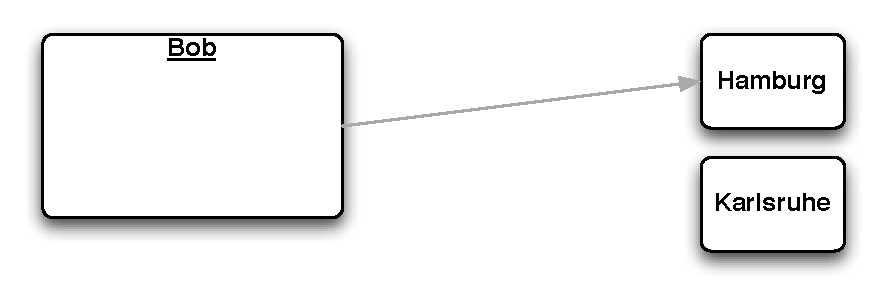
\includegraphics[height=3cm]{Bob1.pdf}

\only<2>{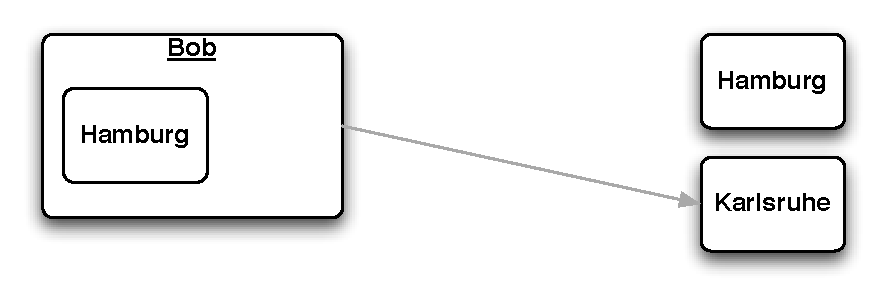
\includegraphics[height=3cm]{Bob2.pdf}}
\end{frame}

\begin{frame}{Alice}
\only<1>{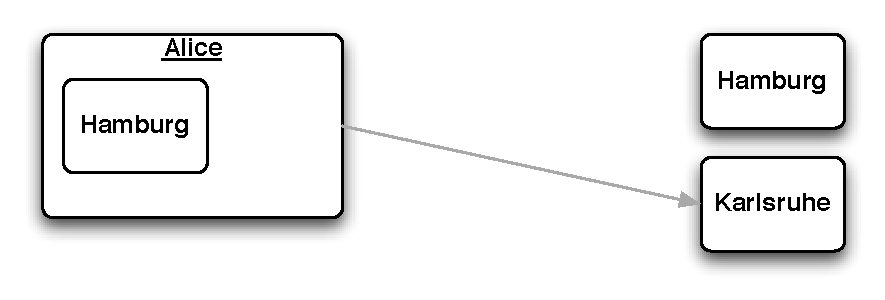
\includegraphics[height=3cm]{Alice1.pdf}}

\only<2>{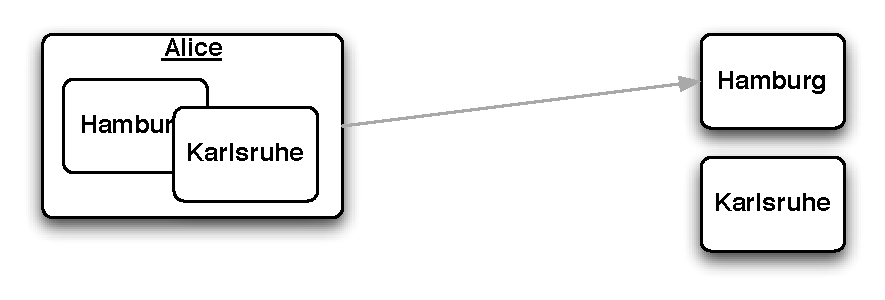
\includegraphics[height=3cm]{Alice2.pdf}}
\end{frame}

% DEMO: ScalaCheck

\begin{frame}{ScalaCheck für Java?}{Erste Ansätze}
	\begin{block}{QuickCheck-Portierung [\href{https://quickcheck.dev.java.net/}{quickcheck.dev.java.net}]}
	\begin{itemize}
		\item Stellt Generatoren für Standardtypen zur Verfügung
		\item Benutzung über \texttt{for}-Schleifen im Unit Test
	\end{itemize}
	\end{block}
	\pause
	\begin{block}{JCheck [\href{http://www.jcheck.org/}{jcheck.org}]}
	\begin{itemize}
		\item Generatoren müssen an jedem Test angegeben werden
		\item Verschachtelte Annotations
		\item Keine Wiederverwendung von Theories
	\end{itemize}
	\end{block}
\end{frame}
\begin{frame}{QuickCheck für Java?}{Neuer Ansatz}
	\begin{block}{JUnit-QuickCheck}
	\begin{itemize}
		\item Eleganter neuer Ansatz
		\item Basiert auf JUnit Theories
		\item Parameter werden mit \texttt{@Forall} annotiert
		\item Vordefinierte Generatoren für Standard-Typen
		\item Steckt noch in den Kinderschuhen
	\end{itemize}
	\end{block}
\end{frame}

% DEMO: junit-quickcheck
\begin{frame}{}
\begin{center}
DEMO
\end{center}
\end{frame}


\begin{frame}{Unterschiede}
	\begin{block}{ScalaCheck}
	\begin{itemize}
		\item Generatoren erzeugen randomisierte Testwerte
		\item Test ist grün nach 100 erfolgreichen Durchläufen
		\item Test ist rot nach 500 unpassenden Eingaben
	\end{itemize}
	\end{block}
	\pause
	\begin{block}{JUnit-QuickCheck}
	\begin{itemize}
		\item Generiert pro Parameter 100 Eingabewerte
		\item Bei 2 Parametern 10.000 Kombinationen, bei drei 1.000.000
		\item Test ist grün, wenn alle passenden Eingaben erfolgreich sind
		\item Test ist rot, wenn kein passender Eingabewert gefunden wurde
	\end{itemize}
	\end{block}
\end{frame}

\begin{frame}{Fazit}

% \glqq{}An example can quickly lead a reader to an intuitive grasp of the desired functionality, but a theory helps make clear which aspects of the example are necessary, and which are arbitrary.\grqq{}
% 
% \hfill[Saff et.al.]

\begin{description}[XX]
\item[Was macht einen guten Unit Test aus?]\hfill\\\pause
Er vermittelt durch \emph{Beispiele} schnell ein intuitives Verständnis.\pause
\item[Was macht eine gute Spezifikation aus?]\hfill\\\pause
Sie beschreibt die zugrundeliegenden Regeln durch \emph{Abstraktion}.\pause
\item[Geht beides zusammen?]\hfill\\\pause
Es gibt kein Entweder-oder; beide Teile sind wichtig.
\end{description}
\end{frame}

\begin{frame}
\begin{center}\Huge
Das war's!
\end{center}
\pause
\vspace{.1cm}
\begin{flushright}\Huge
\itshape Wirklich!
\end{flushright}
\end{frame}

\begin{frame}{Vielen Dank!}

	Code \& Folien auf GitHub:
	\begin{center}
		\url{https://github.com/marcphilipp/xpdays2010/}
	\end{center}

\begin{columns}[t] 
\begin{column}{4.6cm} 
	\begin{block}{Nicole}
        \begin{description}[Twitter]
		\item[E-Mail]  \href{mailto:nicole@andrena.de}{\texttt{nicole@andrena.de}}
		\item[Twitter] \href{http://twitter.com/NicoleRauch}{\texttt{@NicoleRauch}}
        \end{description}
	\end{block}
\end{column} 
\begin{column}{4.6cm} 
	\begin{block}{Marc}
        \begin{description}[Twitter]
		\item[E-Mail]  \href{mailto:marc@andrena.de}{\texttt{marc@andrena.de}}
		\item[Twitter] \href{http://twitter.com/marcphilipp}{\texttt{@marcphilipp}}
        \end{description}
	\end{block}
\end{column} 
\end{columns}
\end{frame}

